% =====================================================================
% VERSION ENSAE, REDUCTION SFE (phase 3, 1er octobre 2026) : chapitre 1, risque cyber, DORA et cadre prudentiel.
% Copie a texte constant de chapitres/02b_cadre_cyber_dora.tex (lignes 1 a 682) puis chapitres/04_cadre_reglementaire.tex (en entier, devenu la section 1.6).
% Ne changent que les titres et les renvois repares, listes dans
% reduction/phase3.md.
% Lu par main_ensae.tex seul : ne jamais le faire lire par main_institut.tex,
% qui garde chapitres/.
% =====================================================================

% =====================================================================
% CHAPITRE 1 : RISQUE CYBER, RESILIENCE NUMERIQUE ET BESOIN DE CAPITAL.
%
% CE CHAPITRE SUIT LE PLAN ARRETE PAR KELIAN. Cinq sections, de la definition du risque a la
% problematique, sur le modele progressif du chapitre 1 de F. Dountio (ENSAE, 2026).
%
% CE QU'IL ABSORBE, ET C'EST LA DECISION DE STRUCTURE LA PLUS LOURDE DU FICHIER. Le plan met
% DORA en section 4 et la problematique en 5.3, or ces deux contenus vivent aujourd'hui dans
% 04_cadre_reglementaire.tex et 02_introduction.tex. SI CE CHAPITRE EST RETENU :
%   - 02_introduction.tex doit disparaitre ou se reduire a ce que 2b.5.3 ne reprend pas. Sa
%     section LUCY (sec:lucy) est reprise ici en section 3 et NE DOIT PAS figurer deux fois ;
%   - 04_cadre_reglementaire.tex doit se reduire a la seule articulation avec Solvabilite II,
%     le cadre DORA lui-meme passant ici. Son label chap:reglementaire doit survivre, cinq
%     chapitres le citent.
% Ne pas compiler le document avec ce chapitre ET les deux autres en l'etat : le lecteur lirait
% deux fois la meme lecture de marche et deux fois les cinq piliers.
%
% LES TROIS SOURCES DE CONTEXTE ET LEUR STATUT. Les valeurs 2026 de la cartographie France
% Assureurs, du barometre CESIN et de l'etude LUCY sont TRANSCRITES dans config.py sous
% CARTO_FA_2026, CESIN_2026 et LUCY_2026, au statut de CITATION EXTERNE NON RECALCULABLE. Le
% depot ne detient aucune de ces donnees d'origine : il ne peut que verifier la fidelite de la
% recopie, ce que font les scripts 63 (LUCY) et 103 (cartographie et barometre). Aucune n'entre
% dans une calibration et aucune ne porte un montant de capital. NE PAS ecrire une valeur de ces
% sources directement ici : elle echapperait au harnais, ce qui est la classe de defaut qui a
% produit les queues Bale et le Hill a 1,42.
%
% LES FIGURES SONT EXTRAITES DES RAPPORTS, comme les trois figures LUCY, et vivent dans
% memoire_cascade/figures_externes/, exception declaree du projet. Son README doit etre complete
% pour chaque figure ajoutee : provenance, page, recadrage. L'AUTORISATION DE REPRODUCTION EST
% ACQUISE POUR TOUTES : accordee par Hugo Rapior le 17 septembre pour les figures LUCY, puis
% etendue par lui le 19 septembre a la cartographie France Assureurs, au barometre CESIN et a la
% carte Avast. Ne pas rouvrir.
%
% AUCUNE FIGURE EN PLEINE PAGE. La macro de figure cle est interdite depuis le 15 septembre.
% Figures en ligne, 5 a 9 cm imprimes.
% =====================================================================

\chapter{Risque cyber, DORA et cadre prudentiel}
\label{chap:cadre-cyber-dora}
\label{part:contexte}



%======================================================================
\section{Pertes, propagation et dépendance}
\label{sec:risque-cyber}

\subsection{Définition et périmètre du risque cyber}
\label{subsec:definition-cyber}
% HARNAIS-HORS-SECTION: section de definitions, sans valeur chiffree issue d'un calcul du projet.

Le risque cyber désigne les pertes liées à une défaillance des systèmes d'information, malveillante
ou non, qui touche la confidentialité des données, leur intégrité ou la disponibilité des services.
L'\emph{incident} couvre tout événement qui affecte la sécurité d'un système, erreurs humaines et
pannes comprises, tandis que la \emph{cyberattaque} en désigne le sous-ensemble intentionnel, abouti
et à impact significatif \citep{cesin2026}. DORA retient la notion la plus large. Son champ, celui
de l'incident lié aux technologies de l'information et de la communication, couvre ainsi une mise à
jour défectueuse qui immobilise un système, même en l'absence de tout adversaire. Nous retenons les pertes propres à l'entité, quelle que soit l'intention, dans le périmètre défini en introduction.

Les conséquences financières dépendent de l'incident : interruption d'activité,
restauration des systèmes ou gestion d'une fuite de données. Un même événement peut en produire
plusieurs. La défaillance d'un prestataire ajoute une dépendance commune entre ses clients.

\begin{figure}[H]\centering
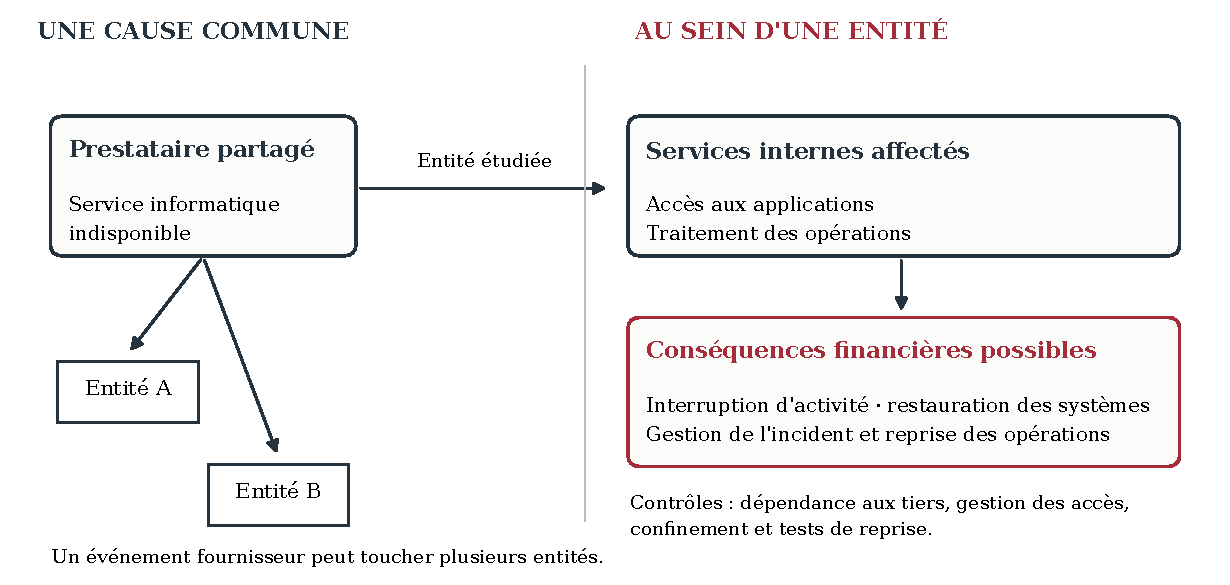
\includegraphics[width=\textwidth]{figures_pedagogie/incident_et_controles.pdf}
\caption{Du service informatique indisponible aux pertes opérationnelles. Ce scénario générique distingue un fournisseur commun à plusieurs entités des conséquences à l'intérieur d'une entité. Les contrôles cités peuvent en limiter les effets ; leur efficacité n'est pas estimée par ce dessin.}
\label{fig:incident-controles}
\end{figure}

La figure~\ref{fig:incident-controles} sépare deux niveaux. À gauche, une cause commune peut
atteindre plusieurs clients. À droite, une seule entité peut subir plusieurs conséquences
du même événement. C'est ce second niveau que décrit la propagation entre piliers ; l'événement
doit rester compté une seule fois dans sa fréquence annuelle.

\subsection{Incidents individuels et chocs de cause commune}
\label{subsec:chocs-cause-commune}
% HARNAIS-HORS-SECTION: section conceptuelle, aucune valeur chiffree.

La compromission d'un prestataire partagé peut produire une \emph{accumulation} : plusieurs
entités sont touchées par la même cause. À l'intérieur d'une entité, les contrôles peuvent aussi
se dégrader ensemble. Une dépendance mal maîtrisée au prestataire, des tests de reprise insuffisants
et une détection tardive peuvent ainsi aggraver les conséquences d'un événement. Nous représentons
cette dépendance entre contrôles par les piliers, au niveau de l'entité étudiée.

La propagation a un sens. Un pilier dont la défaillance entraîne les autres n'appelle pas la même
remédiation qu'un pilier qui subit la leur, alors que les statistiques disponibles n'enregistrent
qu'une co-occurrence. Nous construisons au chapitre~\ref{chap:cascade} la propagation dirigée qui distingue ces deux situations, avant d'étudier au chapitre~\ref{ch:identifiabilite} ce que les données
permettent d'en identifier.

\subsection{Quatre cas de référence}
\label{subsec:cas-cyber}
% HARNAIS-HORS-SECTION: section descriptive, les seuls nombres sont des millesimes d'incidents
% publics et des ordres de grandeur de presse.

Les quatre incidents publics suivants illustrent la propagation, les causes communes et la
dépendance à un prestataire. Ils servent à préciser le périmètre ; ils ne calibrent pas à eux seuls
la matrice de transmission entre piliers.

WannaCry, en $2017$, montre l'échelle de la propagation. Ce rançongiciel auto-propagable exploitait
une faille du protocole de partage de fichiers de Windows. Il a touché en quelques jours des
organisations de dizaines de pays, dont des hôpitaux britanniques et des chaînes de production.
Près d'un an après la divulgation de la faille, un éditeur de sécurité bloquait encore des dizaines
de millions de tentatives d'exploitation \citep{avast2018wannacry}. Ces tentatives ne sont pas des
sinistres : elles montrent qu'une vulnérabilité unique crée une exposition commune et durable.

NotPetya, en $2017$, montre la propagation par un prestataire. Ce logiciel destructeur, diffusé par
la mise à jour d'un logiciel comptable ukrainien, a paralysé pendant plusieurs semaines les réseaux
de groupes internationaux. L'incident naît chez un prestataire (P4, prestataires tiers), se propage faute de
cloisonnement des accès (P1, gouvernance) et met la gestion de crise à l'épreuve (P2, gestion des incidents). Son traitement
assurantiel a donné lieu à des contentieux sur l'exclusion de guerre : un sinistre cyber peut être
avéré sans être couvert.

MOVEit, en $2023$, montre l'accumulation. Une vulnérabilité d'un logiciel de transfert de fichiers,
exploitée par un groupe criminel, a permis de dérober des données chez des milliers d'organisations,
souvent atteintes par leurs propres prestataires. Une seule défaillance tierce produit de nombreux
sinistres simultanés. Nous l'utilisons comme expérience naturelle au
chapitre~\ref{ch:identifiabilite}.

CrowdStrike, en $2024$, montre la dépendance sans adversaire. Une mise à jour défectueuse d'un
logiciel de sécurité a bloqué des millions de postes dans le transport aérien, la banque et la
santé. L'incident relève de la dépendance à un prestataire (P4, prestataires tiers) et de l'absence de déploiement
progressif (P3, tests de résilience). Il entre dans le champ de DORA, et un périmètre restreint aux attaques manquerait
une part du risque que le règlement vise.

Ces cas motivent une représentation de la propagation et des causes communes. Pour un incident,
décrire les domaines touchés ensemble et décrire leur ordre d'atteinte sont deux informations
distinctes ; le modèle du chapitre~\ref{chap:cascade} les sépare.

\section{Limites de l'assurabilité et de la capitalisation du risque cyber}
\label{sec:assurabilite-capital}

\subsection{Fréquence, sévérité et contrat d'assurance}
\label{subsec:frequence-severite-contrat}
% HARNAIS-HORS-SECTION: section de cadrage actuariel, aucune valeur chiffree du projet.

On décompose la charge annuelle d'un risque en un nombre d'événements et un coût par événement,
c'est-à-dire la fréquence et la sévérité. Les mêmes mesures ne réduisent pas les deux, la
sensibilisation des collaborateurs agissant sur la fréquence et une capacité de reprise sur la
sévérité. Nous appliquons cette décomposition à l'écart de capital entre états de conformité
(chapitre~\ref{chap:resultats}).

Le contrat d'assurance transforme la perte. La \emph{franchise} laisse à l'assuré la première
tranche du sinistre et la \emph{capacité} plafonne l'engagement de l'assureur, si bien qu'une
charge indemnisée et une perte brute ne se comparent ni en niveau ni en quantile. Sur des données
agrégées, une baisse de franchise et une aggravation de la menace produisent le même signal, à
savoir une charge indemnisée qui monte. On retrouve cette situation au
chapitre~\ref{ch:identifiabilite}, à l'échelle des piliers, et nous la traitons de la
même façon, en bornant ce que la donnée ne sépare pas.

\subsection{Conditions d'assurabilité et asymétrie d'information}
\label{subsec:dependance-accumulation}
% HARNAIS-HORS-SECTION: section de cadrage, aucune valeur chiffree du projet.

Le risque cyber met à l'épreuve les conditions de l'assurabilité. La défaillance d'un prestataire commun accroît la dépendance des pertes et limite la mutualisation. Une attaque ciblée reste incertaine pour la victime ; son caractère intentionnel ne supprime pas à lui seul l'aléa assurable. L'historique
manque en outre là où se joue la quantification. L'asymétrie d'information entre assureur et assuré sur
l'état réel du système d'information renforce enfin l'aléa moral et l'anti-sélection. DORA agit sur
ce dernier point, car le registre des accords avec les prestataires, la notification des incidents
majeurs et les tests de résilience rendent la maîtrise du risque observable. Une méthode qui traduit
cette maîtrise en capital pourra exploiter cette information.

\subsection{Rareté des données extrêmes et limite de l'historique français}
\label{subsec:donnees-extremes}
% HARNAIS-HORS-SCRIPT: le niveau reglementaire 99,5 % est pose par la directive ; le recul
% de 20 % des sinistres et les millesimes 2020-2022 viennent d'analyses de sinistralite
% europeennes citees en bibliographie, que le depot ne detient pas et ne recalcule pas.

Le besoin ORSA étudié est le quantile à $99{,}5\,\%$ de la charge annuelle, dépassé une année
sur deux cents. Il dépend donc des sinistres les plus lourds, pour lesquels la donnée française est
presque vide (section~\ref{sec:marche-cyber-francais}). Pour estimer une queue par dépassement de
seuil, on ne retient que les pertes au-dessus d'un montant élevé, et il faut un effectif suffisant
au-delà de ce seuil, ce que l'historique national n'offre pas. Une estimation sur cette base serait
instable et sous-estimerait le risque, faute d'avoir observé les pertes qui le déterminent. C'est
pourquoi nous calibrons la sévérité sur une base internationale (chapitre~\ref{chap:donnees}).

Cette rareté ne traduit pas une protection du marché français. Les sinistres cyber européens
ont certes reculé d'environ $20\,\%$ en $2024$, mais restent près d'un tiers au-dessus des exercices
$2020$ à $2022$ \citep{marsh2025}, et le marché britannique est décrit comme plus exposé aux
sinistres sévères \citep{dsit2025}.

\section{Marché français de la cyberassurance}
\label{sec:marche-cyber-francais}
% SOURCES-SCRIPTS: 63

L'étude LUCY de l'AMRAE, dont l'édition $2026$ couvre l'exercice $2025$, observe le marché français
sur $20\,996$ polices et $1\,251$ sinistres déclarés, recueillis auprès de douze courtiers et d'un
assureur \citep{amraeLucy2026}. La série, engagée en $2019$, compte sept exercices comparables. Nous
avons co-écrit l'analyse actuarielle de cette édition \citep{RapiorKaddouri2026}. Ses valeurs sont
reprises comme des citations externes, que nous ne pouvons pas recalculer, et n'entrent ni dans le
modèle ni dans le calcul d'un montant de capital.

Un script du dépôt contrôle toutefois la fidélité
de la recopie. Le rapport des sinistres aux primes redonne la série publiée des ratios, la somme
des classes de taille redonne la charge annuelle sur les sept exercices, et chaque multiplicateur
cité se retrouve à partir des niveaux qui l'encadrent. Ces contrôles ne portent ni sur la collecte
ni sur le périmètre de l'étude, qui relèvent de ses auteurs.

La charge indemnisée s'élève à $83{,}2$~M\euro{} en $2025$ contre $54{,}5$ l'exercice précédent, soit
$+53\,\%$. Nette de franchise et plafonnée par la capacité, elle ne se compare pas à la perte brute
d'une entité, que nous modélisons. Entre $2024$ et $2025$, le nombre d'entreprises assurées croît de
$49\,\%$, mais les primes reculent de $3\,\%$. Le ratio sinistres sur primes remonte depuis
deux exercices, de $12\,\%$ en $2023$ à $27\,\%$, loin des $169\,\%$ de $2020$. Le marché se diffuse donc par le volume plutôt que par le budget :
davantage d'entreprises sont couvertes, pour une prime moyenne plus faible, au moment où la
sinistralité remonte (figure~\ref{fig:lucy-ratio}). Le recul du taux de prime atteint $33\,\%$ pour
les grandes entreprises et $23\,\%$ pour les entreprises de taille intermédiaire. Cet assouplissement
ne repose sur aucune amélioration mesurée de la maîtrise du risque.

\begin{figure}[H]
\centering
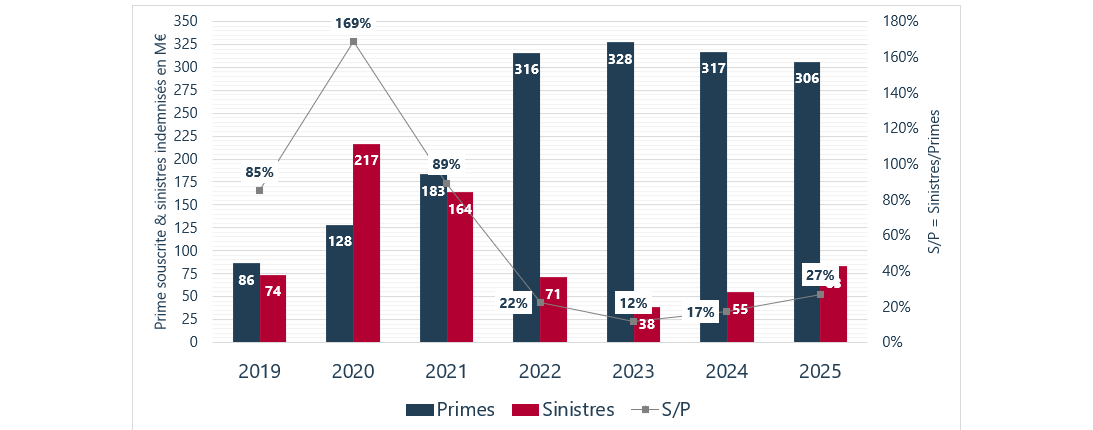
\includegraphics[width=0.80\textwidth]{figures_externes/lucy_primes_sinistres_ratio.png}
\caption{Primes souscrites, sinistres indemnisés et ratio sinistres sur primes, $2019$--$2025$. La
sinistralité remonte depuis deux exercices alors que les primes reculent. Source :
rapport LUCY 2026, Nexialog Consulting \citep{RapiorKaddouri2026}.}
\label{fig:lucy-ratio}
\end{figure}

La hausse du ratio recouvre deux régimes opposés. En $2024$, les sinistres sont moins nombreux
($\times 0{,}73$) mais deux fois plus lourds ($\times 1{,}96$). En $2025$, ils sont presque
trois fois plus nombreux ($\times 2{,}79$) pour un coût moyen divisé par deux ($\times 0{,}55$). Seule la
décomposition de la charge en nombre et coût moyen sépare ces deux situations, qui n'appellent pas
les mêmes mesures. Le tableau donne chaque terme sous la forme d'un multiplicateur de la valeur de
l'année précédente.

\begin{center}\small
\renewcommand{\arraystretch}{1.2}
\begin{tabular}{@{}l r r r l@{}}
\toprule
& \textbf{nombre} & \textbf{sinistre moyen} & \textbf{charge} & \textbf{régime} \\
\midrule
Marché, exercice $2024$ & $\times 0{,}73$ & $\times 1{,}96$ & $\times 1{,}43$ & sévérité \\
Marché, exercice $2025$ & $\times 2{,}79$ & $\times 0{,}55$ & $\times 1{,}53$ & fréquence \\
\midrule
\multicolumn{5}{@{}l}{\emph{Exercice $2025$, par bloc}} \\
grandes entreprises & $\times 1{,}24$ & $\times 0{,}82$ & $\times 1{,}02$ & absorbé \\
bloc intermédiaire & $\times 2{,}14$ & $\times 1{,}65$ & $\times 3{,}53$ & les deux \\
micro-entreprises & $\times 9{,}52$ & $\times 0{,}73$ & $\times 6{,}97$ & nombre seul \\
\bottomrule
\end{tabular}
\end{center}

\vspace{2pt}
\noindent Le bloc intermédiaire est le seul segment où le nombre et le coût moyen augmentent
ensemble, d'où une charge multipliée par $3{,}53$. Ces multiplicateurs portent sur le \emph{nombre}
de sinistres, un total, et non sur la fréquence, qui le rapporte au nombre d'assurés. L'égalité
charge $=$ nombre $\times$ coût moyen n'est exacte qu'avec le nombre.

La divergence entre le prix et le risque ne se répartit pas uniformément : le segment dont la
sinistralité progresse le plus n'est pas celui dont le tarif se redresse. Les multiplicateurs les
plus forts portent sur les micro-entreprises, dont la part dans la charge totale reste marginale ;
un multiplicateur hiérarchise des dynamiques, non des enjeux.

La limite qui engage notre modélisation se situe dans la queue. Deux exercices sur sept ne comptent
aucun sinistre de la classe de 10 à 40~M\euro{}, et un exercice y enregistre
$135$~M\euro{}. En $2025$, cette classe représente $19$~M\euro{}, pour un seul sinistre au-delà de
$10$~M\euro{} (figure~\ref{fig:lucy-taille}). L'historique national s'arrête avant le haut de la distribution. 

\begin{figure}[H]
\centering
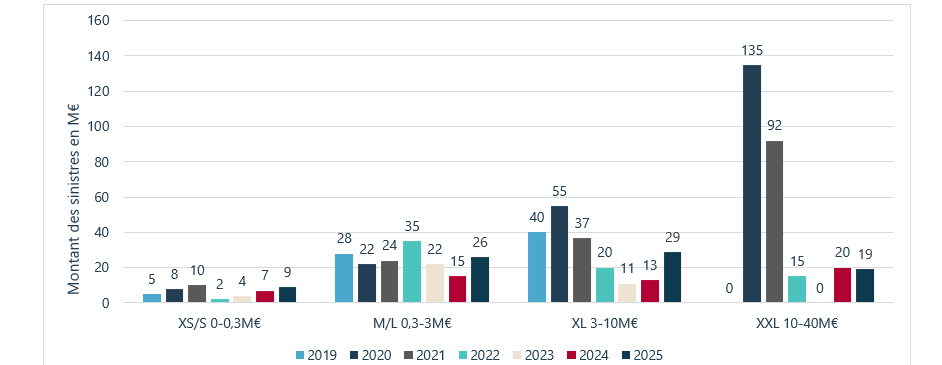
\includegraphics[width=0.80\textwidth]{figures_externes/lucy_taille_des_sinistres.png}
\caption{Charge indemnisée par classe de taille de sinistre, $2019$--$2025$. La classe la plus
haute est vide deux exercices sur sept : l'historique national s'arrête avant le haut de la
distribution.
Source : rapport LUCY 2026, Nexialog Consulting \citep{RapiorKaddouri2026}.}
\label{fig:lucy-taille}
\end{figure}

\section{Le règlement DORA}
\label{sec:dora}
% HARNAIS-HORS-SECTION: section reglementaire. Les seuls nombres sont des millesimes, des
% numeros d'articles et des references de textes, aucun ne provient d'un calcul du projet.

\subsection{Cadre réglementaire européen du cyber}
\label{subsec:cadre-reglementaire-europeen}
% HARNAIS-HORS-SECTION: section reglementaire. Les nombres sont la date d'entree en
% application, des millesimes et des numeros officiels de textes. Ce sont des donnees de droit.

Quatre textes européens encadrent le risque cyber. La directive NIS~2
\citep{NIS2Directive2022}, relative à la sécurité des réseaux et des systèmes d'information, impose
des exigences de sécurité et de notification aux entités essentielles et importantes. Elle rend
également l'organe de direction responsable des mesures de gestion du risque. Le règlement général
sur la protection des données \citep{RGPD2016} encadre les données personnelles, la directive sur la
résilience des entités critiques \citep{REC2022} la continuité des fonctions sociétales vitales. Le
règlement sur la cyberrésilience \citep{CRA2024} couvre enfin la sécurité des produits numériques.
Aucun n'est propre au secteur financier.

Le règlement DORA \citep{DORA2022} comble ce manque. Entré en application le $17$ janvier $2025$, il
s'adresse à une vingtaine de catégories d'entités financières, dont les entreprises d'assurance, et
leur demande de résister à l'incident, d'y réagir et de s'en rétablir. 

Nous ne modélisons que DORA, car il est le seul de ces textes à découper la résilience en piliers
dont la défaillance pourra se lire dans les incidents notifiés. Les cadres de l'intelligence
artificielle et de l'identité numérique ne sont pas traités. Le règlement sur la cyberrésilience,
applicable à partir de décembre~$2027$, agira sur la fréquence future des vulnérabilités. Notre calibration l'estime sur l'historique et ne la projette pas.

\subsection{Les cinq piliers de DORA}
\label{subsec:cinq-piliers-dora}
% HARNAIS-HORS-SECTION: section reglementaire. Les nombres sont les etiquettes P1 a P5, les
% numeros d'articles du reglement et les delais qu'il fixe. Ce sont des donnees de droit.

Le règlement organise la résilience en cinq domaines, notés P1 à P5, que nous appelons \emph{piliers}.
\begin{itemize}[leftmargin=1.4em,itemsep=2pt]
\item P1, gouvernance du risque lié aux technologies (articles~$5$ à~$16$) : responsabilité non
      délégable de l'organe de direction, cartographie des actifs et des dépendances critiques,
      contrôle interne continu.
\item P2, gestion, classification et notification des incidents (articles~$17$ à~$23$) : notification initiale dès que possible, sous quatre heures après classification majeure et au plus tard vingt-quatre heures après prise de connaissance. Si la classification intervient après ce délai, la notification suit sous quatre heures. Le rapport intermédiaire est dû sous soixante-douze heures après la notification initiale, le rapport final sous un mois après le rapport intermédiaire ou sa dernière mise à jour \citep{eu2025_301}.
\item P3, tests de résilience opérationnelle numérique (articles~$24$ à~$27$), dont des tests de
      pénétration guidés par la menace (TLPT), au moins tous les trois ans, pour les entités
      significatives (article~$26$).
\item P4, gestion du risque lié aux prestataires tiers (articles~$28$ à~$44$) : registre
      d'informations des contrats, clauses impératives de l'article~$30$, stratégie de sortie et
      surveillance des prestataires critiques. Leur chaîne de sous-traitance est prise en compte sans limite générale au troisième rang.
\item P5, partage d'informations sur les cybermenaces (article~$45$), volontaire et encadré, le
      pilier le moins utilisable dans un calibrage actuariel.
\end{itemize}
Ces piliers ne sont pas indépendants, car un incident qui touche l'un dégrade la capacité de l'entité à tenir les autres (sous-section~\ref{subsec:chocs-cause-commune}). Nous formalisons cette dépendance au chapitre~\ref{chap:cascade}.

\subsection{Prestataires TIC, concentration et propagation du risque}
\label{subsec:risque-tiers-dora}
% SOURCES-SCRIPTS: 103

La sous-traitance informatique du secteur financier est concentrée sur un petit nombre de
fournisseurs, si bien qu'une défaillance chez l'un d'eux atteint de nombreuses entités sans faute de
leur part. DORA instaure pour cette raison une surveillance directe des prestataires critiques, ce qui
est nouveau dans l'architecture prudentielle européenne. Le premier bilan des notifications montre
le poids des prestataires. En $2025$, les sociétés de gestion ont adressé à l'Autorité des marchés
financiers $47$ notifications initiales, dont $31$ incidents majeurs confirmés, parmi lesquels $27$,
soit $87\,\%$, trouvent leur origine chez un prestataire \citep{amf2026incidents}.

Cette part dit d'où viennent les incidents ; elle ne fournit pas de probabilité de transfert entre piliers et ne calibre aucun paramètre du modèle. Les notifications initiales précèdent la confirmation du caractère majeur : l'écart avec les
incidents confirmés est celui d'un seuil de matérialité, et la collecte réglementaire ne retiendra que
les incidents au-dessus de ce seuil.

Pour la modélisation, l'exigence la plus utile est le registre d'informations. En recensant les
contrats TIC critiques et leurs chaînes de sous-traitance, il produit une donnée sur la concentration
technologique que l'évaluation interne des risques ne savait pas chiffrer. Il ne couvre que
la dépendance déclarée et ne dit rien de l'ordre dans lequel les défaillances s'enchaînent
(section~\ref{ch:livrable}).

\subsection{Autorités françaises et supervision}
\label{subsec:supervision-france}
% HARNAIS-HORS-SECTION: section institutionnelle, aucune valeur chiffree.

À notre connaissance, les autorités de supervision ne publient pas de probabilité de propagation entre
piliers. Elles publient des attentes prudentielles et des échelles de maturité, qui sont d'une autre nature. Les
valeurs de propagation du modèle sont donc posées à dire d'expert, puis bornées, et nous ne les
présentons pas comme calibrées sur une source officielle.

\section{Perception du risque et traitement prudentiel}
\label{sec:enjeu-prudentiel}

\subsection{Perception prospective selon France Assureurs et le CESIN}
\label{subsec:france-assureurs-cesin}
% SOURCES-SCRIPTS: 103 63

La cartographie prospective de France Assureurs classe le risque cyber au premier rang pour le
huitième exercice consécutif, avec un score de $4{,}1$ sur $5$ \citep{franceassureurs2026}. Ce score
a culminé à $4{,}48$ en $2022$ et revient à $4{,}10$ en $2026$.
Entre $2025$ et $2026$, il recule de $0{,}45$ point en fréquence anticipée et progresse de
$0{,}25$ point en sévérité : moins d'événements attendus, mais plus lourds. Le cyber n'est pas seul
dans ce régime.

Deux risques seulement de la cartographie gagnent en
sévérité tout en reculant en fréquence. Ce sont le cyber, à $+0{,}25$ point de sévérité pour $-0{,}45$ de
fréquence, et la qualité des données et la conformité des processus informatiques, à $+0{,}30$ pour
$-0{,}20$. Le déplacement le plus fort de l'édition en sévérité appartient à l'environnement
politique, à $+0{,}32$, mais il s'accompagne d'une hausse de fréquence de $+0{,}30$ et relève d'un
autre régime. La cartographie fait par ailleurs figurer un risque de non-conformité et de sanctions
ainsi qu'un risque lié à l'intelligence artificielle. La préoccupation de la profession se déplace de
la menace vers sa gouvernance, qui est l'objet de DORA.

D'après le baromètre du CESIN (Club des experts de la sécurité de l'information et du numérique), qui en donne le constat déclaré \citep{cesin2026}, $40\,\%$ des
entreprises interrogées ont subi au moins une cyberattaque significative en $2025$. Parmi les $159$
qui en ont constaté une, l'hameçonnage est cité par $55\,\%$, l'exploitation d'une faille par
$41\,\%$. Chaque entreprise attaquée cite en moyenne $3{,}3$ vecteurs, contre $4{,}0$ à la vague
précédente, car une attaque n'emprunte presque jamais un chemin unique
(figure~\ref{fig:cesin-vecteurs}). L'attaque indirecte par un tiers pèse $35\,\%$, et sa part monte à
$43\,\%$ dans les grandes entreprises. On reconnaît là le pilier P4, vu par une
source indépendante de ce travail.

\begin{figure}[H]
\centering
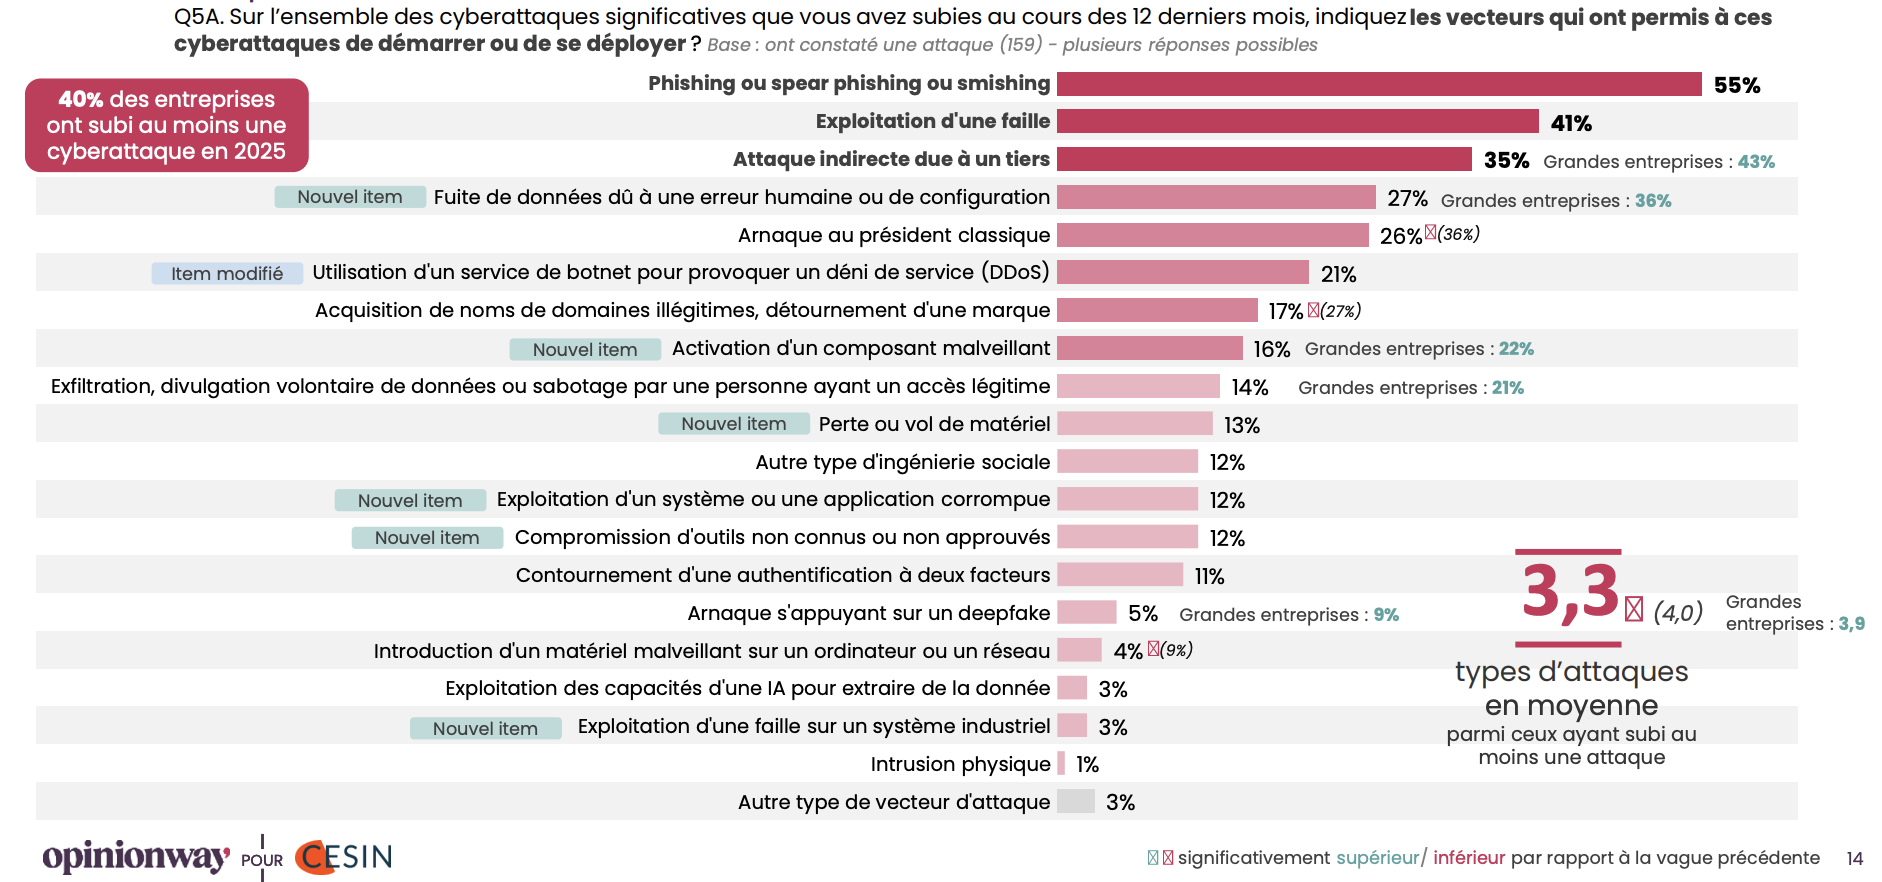
\includegraphics[width=0.78\textwidth]{figures_externes/cesin_2026_vecteurs.png}
\caption{Vecteurs ayant permis aux cyberattaques de démarrer ou de se déployer, exercice $2025$. Les
mentions de droite donnent la part dans les grandes entreprises lorsqu'elle diffère
significativement de la moyenne. Source : baromètre de la cybersécurité des entreprises,
OpinionWay pour le CESIN \citep{cesin2026}.}
\label{fig:cesin-vecteurs}
\end{figure}

Quatre entreprises attaquées sur cinq, soit $81\,\%$, déclarent un impact sur leur activité. Les
conséquences dominantes sont la perturbation de la production, à $28\,\%$, et la perte d'image, à
$26\,\%$, devant la compromission de savoir-faire et la perte de chiffre d'affaires, à $18\,\%$
chacune. La sanction d'une autorité ne concerne que $3\,\%$ des cas. Nous ne modélisons donc pas les pénalités : la non-conformité coûte,
dans le modèle, par les incidents qu'elle laisse passer. La déconnexion de l'entité par ses propres partenaires, citée dans $12\,\%$ des cas,
montre enfin que la dépendance joue dans les deux sens, avec des coûts et des préventions
différents.

\section{Cadre prudentiel et articulation avec DORA}
\label{chap:reglementaire}

% HARNAIS-HORS-SCRIPT: cadre reglementaire : numeros d'articles, delais de notification et seuils cites des textes (DORA, Solvabilite II, Bale). Ce sont des donnees de droit, pas des resultats.

Le risque opérationnel reçoit la même définition dans la banque et dans l'assurance. Il s'agit du
risque de perte résultant de l'inadaptation ou de la défaillance de procédures, de personnels et de
systèmes internes, ou d'événements extérieurs. Il comprend le risque juridique et exclut les risques
stratégique et de réputation.

Les modes de quantification ont cependant divergé. Le secteur bancaire a abandonné les
modèles internes de mesure avancée au profit d'une approche standardisée \citep{bcbs2017}, sans invalider l'approche
par distribution des pertes (LDA, \emph{Loss Distribution Approach}) comme outil de modélisation.
Nous en reprenons les deux marges, fréquence et sévérité, et remplaçons son agrégation par une
cascade dirigée. L'assurance conserve sous Solvabilité~II le choix entre la Formule Standard, des
paramètres propres à l'entreprise et un modèle interne, partiel ou global, approuvé par l'autorité de
contrôle.

Dans la Formule Standard, l'exigence pour risque opérationnel ($SCR_{Op}$) s'ajoute au capital de
solvabilité requis de base ($BSCR$), ajusté de la capacité d'absorption des pertes :
\begin{equation}
SCR = BSCR + Adj + SCR_{Op},
\qquad
SCR_{Op} = \min(0{,}3 \times BSCR,\ Op) + 0{,}25 \times Exp_{ul},
\label{reg:eq:scrop}
\end{equation}
où $Adj$ est l'ajustement pour la capacité d'absorption des pertes, $Exp_{ul}$ les frais annuels des contrats en unités de compte et $Op = \max(Op_{premiums}, Op_{provisions})$ applique des coefficients forfaitaires aux primes et
aux provisions. Cette forme est simplifiée, car l'article~204 du règlement délégué~2015/35 ajoute des
termes de croissance, de la forme $\max\!\left(0;\, 0{,}04 \times \Delta\!\right)$, qui pénalisent
les hausses de primes supérieures à $20\,\%$ d'un exercice à l'autre.

Fondée sur des indicateurs de
volume, l'approche attribue la même exposition à deux assureurs de même volume, quelles que soient la
qualité de leur informatique et leur dépendance à des prestataires critiques. Le $SCR_{Op}$ réglementaire s'ajoute au BSCR sans diversification. Cela n'implique pas qu'un quantile ORSA supplémentaire doive être ajouté en entier : il faut éviter le double compte du risque informatique déjà couvert (\S\ref{sec:agregation-scr}).

Le $SCR_{Op}$ relève des exigences quantitatives (forfaitaires) de Solvabilité~II. Les exigences de gouvernance imposent l'évaluation
interne des risques et de la solvabilité (\emph{Own Risk and Solvency Assessment}, ORSA). Elle
confronte le profil de risque réel aux besoins de solvabilité et admet les scénarios stochastiques
que la Formule Standard ne produit pas. Notre modélisation se situe dans ce cadre. ORSA et DORA
partagent un objet, le risque opérationnel d'origine technologique, l'ORSA pour la continuité
financière, DORA pour la continuité opérationnelle. Nous partons d'états de conformité posés pour quantifier dans l'ORSA ce que celui-ci ne savait que décrire (chapitres~\ref{chap:multietats}
et~\ref{chap:resultats}).

\subsection{De l'approche de mesure avancée à l'approche standardisée}
\label{subsec:ama-sma}
% HARNAIS-HORS-SECTION: cadre reglementaire : numeros d'articles, delais et seuils cites des textes,
% donnees de droit et non resultats.

Sous Bâle~II, les établissements bancaires d'envergure internationale étaient encouragés à développer
des modèles internes, regroupés sous le nom d'approche de mesure avancée (\emph{Advanced Measurement
Approaches}, AMA). Ces modèles reposaient surtout sur l'approche par distribution des pertes (LDA) ou
sur des scénarios. Leur flexibilité a produit des actifs pondérés par le risque très variables d'un
établissement à l'autre, et difficiles à justifier, ce qui a érodé la confiance des superviseurs dans les
ratios déclarés.

La finalisation de Bâle~III, souvent appelée Bâle~IV, remplace les modèles AMA par une approche standardisée.
Dans l'Union européenne, CRR~III s'applique depuis le 1\textsuperscript{er}~janvier~2025. Il faut distinguer
ce texte du standard international de Bâle \citep{CRRIII2024}. Dans ce dernier, l'exigence de
capital opérationnel combine une composante de volume d'activité, le \emph{Business
Indicator Component} ($BIC$), et un facteur d'échelle fondé sur l'historique des pertes internes,
l'\emph{Internal Loss Multiplier} ($ILM$) :
\begin{equation}
ORC = BIC \times ILM,
\qquad
RWA_{Op} = 12{,}5 \times ORC.
\end{equation}
Le \emph{Business Indicator} résume la taille de l'établissement à partir de trois composantes comptables
(intérêts et dividendes, services, activité financière), auxquelles s'appliquent des coefficients
marginaux croissants par tranches. Le profil de risque propre revient par l'$ILM$, qui compare le $BIC$ à
la composante de pertes historiques $LC$, égale à quinze fois la moyenne des pertes opérationnelles
annuelles significatives des dix dernières années. Lorsque la sinistralité est faible par rapport à
l'activité ($LC < BIC$), l'$ILM$ est inférieur à l'unité et réduit l'exigence. Lorsqu'elle est élevée, il
agit comme une pénalité en fonds propres.

Dans l'Union européenne, l'article~312 de CRR~III retient au contraire $ORC=BIC$, sans ajustement
par l'$ILM$. La collecte des pertes subsiste, mais ne multiplie pas cette exigence. Le retrait de
l'AMA n'invalide pas la LDA comme outil de modélisation interne. Nous en reprenons la logique de
distribution des pertes en ORSA, sans la présenter comme une règle bancaire européenne.

\subsection{Critique du module de risque opérationnel de la Formule Standard}
\label{subsec:critique-formule-standard}
% SOURCES-SCRIPTS: 27 67 60 130 47 95 65 136

La charge de l'équation~\eqref{reg:eq:scrop} est examinée ici au regard d'une question précise :
traduire en capital une différence d'état de conformité DORA entre deux entités. Ce n'est pas la
question que le module cherche à résoudre. Il vise une charge simple, comparable d'une entité à
l'autre et peu exposée au risque de modèle, ce qui justifie sa forme forfaitaire au pilier~1. Les
limites relevées ci-dessous portent donc sur son adéquation à l'objet étudié, non sur sa légitimité
réglementaire. Faute de sous-module cyber, l'évaluation de cet objet revient aux modèles internes
et à l'ORSA. Deux propriétés de la formule fondent la critique.

\begin{proposition}[Invariance et homogénéité de la charge forfaitaire]\label{prop:forfait}
Soit $v$ le vecteur des grandeurs de volume d'une entité : primes acquises de l'exercice et de
l'exercice précédent, provisions techniques, $BSCR$ et $Exp_{ul}$. Soit $\theta$ les paramètres
de sa loi de perte opérationnelle : fréquence, détection, propagation et accumulation.
\begin{enumerate}[label=(\roman*)]
\item $SCR_{Op}$ est une fonction de $v$ seule : à $v$ fixé, il ne dépend pas de $\theta$.
\item $SCR_{Op}$ est positivement homogène de degré un : $SCR_{Op}(c\,v)=c\,SCR_{Op}(v)$ pour tout
$c>0$, termes de croissance et plafond compris.
\end{enumerate}
\end{proposition}

\begin{proof}
(i) L'article~204 du règlement délégué~2015/35 n'emploie comme arguments que les composantes de
$v$. (ii) Chaque terme de $Op_{premiums}$ et de $Op_{provisions}$ est de la forme $\alpha x$ ou
$\max(0,\alpha x-\beta y)$. Ici $\alpha,\beta\ge0$ sont fixés et $x,y$ sont des composantes de $v$. Ces
fonctions sont positivement homogènes de degré un. Le maximum, le minimum et la somme de telles
fonctions le restent, d'où l'homogénéité de $\min(0{,}3\,BSCR,\ Op)+0{,}25\,Exp_{ul}$.
\end{proof}

La propriété~(i) implique qu'à volume égal l'écart de charge entre un état conforme et un état non
conforme est nul. La propriété~(ii) fixe à un l'élasticité de la charge lorsque tous les volumes,
$BSCR$ compris, sont multipliés par le même facteur. Le
tableau~\ref{tab:critique-formule-standard} en déduit six limites pour la question étudiée et
indique, pour chacune, la réponse étudiée dans la suite du mémoire. Les valeurs citées
sont établies aux chapitres de renvoi.

\begin{table}[H]\centering\small
\begingroup
\definecolor{reperecritique}{HTML}{A52D39}
\definecolor{reperereponse}{HTML}{14828B}
\renewcommand{\arraystretch}{1.28}
\begin{tabularx}{\textwidth}{@{}>{\raggedright\arraybackslash}p{.15\textwidth}>{\raggedright\arraybackslash}X>{\raggedright\arraybackslash}X>{\raggedright\arraybackslash}X@{}}
\toprule
\textbf{Limite} & \textbf{Constat (texte réglementaire)} & \textcolor{reperecritique}{\textbf{Conséquence pour la question étudiée}} & \textcolor{reperereponse}{\textbf{Réponse étudiée}} \\
\midrule
L1 · Indicateur de volume
& Arguments : primes, provisions, BSCR et frais des unités de compte ; le terme de croissance pénalise une hausse des primes, non du risque.
& Écart de charge nul entre états de même volume (proposition~\ref{prop:forfait}, tableau~\ref{tab:benchmark-sf}) ; une remédiation ne modifie pas le capital.
& Quatre canaux de conformité dans la loi de perte (chapitre~\ref{chap:multietats}). \\
\addlinespace
L2 · Proportionnalité à la taille
& Charge homogène de degré un en volume.
& Lien taille--charge fixé par convention. Le modèle lit la taille dans deux entrées (exposant de fréquence estimé sur les grandes institutions, $0{,}087$ en sévérité) ; le capital s'obtient en recalculant le quantile.
& Fréquence et sévérité lues à la taille, exposant de fréquence estimé sur les grandes institutions (\S\ref{sec:ancrage}). \\
\addlinespace
L3 · Absence de loi de perte
& Coefficients fixés par le règlement, sans modèle de perte propre à l'entité.
& Le quantile à $99{,}5\,\%$ de la perte opérationnelle n'est pas lisible ; la queue lourde ($\hat\xi=0{,}595$) n'est pas représentée.
& Modèle fréquence-sévérité à queue de Pareto généralisée (chapitre~\ref{chap:socle}). \\
\addlinespace
L4 · Plafond relatif
& Composante hors frais des unités de compte plafonnée à $0{,}3\,BSCR$.
& Pour l'assureur non-vie~A ($Adj=0$ posé), la marge sous le plafond, $50{,}8$~M\euro, est dépassée par le besoin non conforme ($112{,}1$) mais pas par l'écart de contagion ($34{,}9$, soit $0{,}69$ fois).
& Agrégation de l'écart en ORSA (\S\ref{sec:agregation-scr}). \\
\addlinespace
L5 · Absence de structure de dépendance
& Charge scalaire ajoutée au BSCR, sans dépendance entre domaines de contrôle.
& Le comparateur à copule gaussienne figée construit ici restitue $62\,\%$ de l'écart simulé (\S\ref{sec:benchmark}) ; deux matrices transposées, non distinguées par les statistiques disponibles, donnent des capitaux différents.
& Cascade dirigée et identification partielle (chapitres~\ref{chap:cascade} et~\ref{chap:partielle}). \\
\addlinespace
L6 · Absence d'historique de pertes
& Aucun terme de sinistralité, à la différence du standard de Bâle avec $ILM$ ; CRR~III ne le retient pas (\S\ref{subsec:ama-sma}).
& Les notifications et registres produits au titre de DORA n'ont pas d'effet sur la charge.
& Valeur d'information d'un registre d'incidents (\S\ref{ch:livrable}). \\
\bottomrule
\end{tabularx}
\endgroup
\caption{Six limites du module de risque opérationnel pour la question étudiée, et réponses
examinées dans le mémoire. L1 et L2 découlent de la proposition~\ref{prop:forfait} ; L3 à L6 tiennent
à la construction du module.}
\label{tab:critique-formule-standard}
\end{table}

La figure~\ref{fig:critique-formule-standard} illustre la différence d'objet entre les deux
approches. La charge forfaitaire est une fonction du volume ; le besoin de capital de l'ORSA est un
quantile d'une loi de perte que l'état de conformité déplace.

\begin{figure}[H]\centering
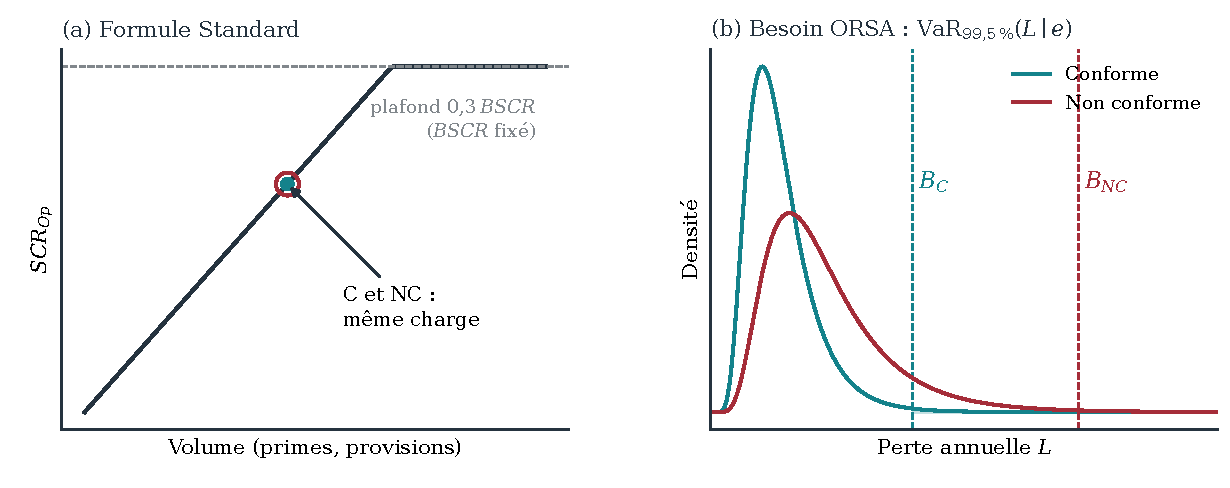
\includegraphics[width=\textwidth]{figures_pedagogie/critique_formule_standard.pdf}
\caption{Deux objets distincts. (a)~Charge de la Formule Standard en fonction du volume, à $BSCR$
fixé (le plafond $0{,}3\,BSCR$ ne bouge donc pas) : deux entités de même volume reçoivent la même
charge, quel que soit leur état de conformité. (b)~Besoin
de capital au sens de l'ORSA : quantile à $99{,}5\,\%$ de la perte annuelle, déplacé par l'état de
conformité. Illustration sans valeur estimée ; les valeurs du périmètre étudié figurent au
tableau~\ref{tab:benchmark-sf}.}
\label{fig:critique-formule-standard}
\end{figure}

Ces limites ne plaident pas pour remplacer le forfait du pilier~1, dont la comparabilité entre
entités reste un objectif prudentiel propre. Elles délimitent ce qu'il ne peut pas exprimer : la
réponse étudiée relève du pilier~2, où l'ORSA admet une loi de perte propre à l'entité et des
scénarios de conformité.

\subsection{Recouvrement de Solvabilité~II et de DORA}
\label{subsec:orsa-dora-detail}
% Condense le 26 octobre 2026 : le tableau comparatif repetait les delais et obligations du
% \S1.4.2 et indiquait des chaines de sous-traitance limitees au rang 3, contraire au \S1.4.2.

Outre leur finalité, financière pour l'un et opérationnelle pour l'autre, les deux cadres diffèrent
par leurs critères de proportionnalité. Le forfait de Solvabilité~II utilise des volumes ; DORA tient
aussi compte de la taille, du profil de risque et de la complexité des activités (article~4). La petite taille ne suffit pas à ouvrir le cadre simplifié : le champ et les exclusions de DORA se lisent aux articles~2 et~16.

DORA apporte à l'ORSA trois éléments décrits au \S\ref{subsec:cinq-piliers-dora} : un cadre de
gestion des contrôles, une notification standardisée des incidents majeurs et un
registre des dépendances aux prestataires. Ils répondent à trois limites des ORSA fondés sur des
cartographies d'experts. Ces ORSA traitent les risques informatiques à part des risques financiers et
assurantiels, sans corrélation modélisée. Ils manquent de données de sinistralité qualifiées pour les
événements rares et lourds, et leurs tests de résistance omettent la propagation d'une panne
chez un fournisseur partagé. Ce travail se place dans ce recouvrement. Il croise plusieurs sources
indépendantes (PRC, SAS OpRisk Global, Hackmageddon) en déclarant l'incertitude résiduelle, et
représente la propagation entre domaines de contrôle.
